\documentclass[1p]{elsarticle_modified}
%\bibliographystyle{elsarticle-num}

%\usepackage[colorlinks]{hyperref}
%\usepackage{abbrmath_seonhwa} %\Abb, \Ascr, \Acal ,\Abf, \Afrak
\usepackage{amsfonts}
\usepackage{amssymb}
\usepackage{amsmath}
\usepackage{amsthm}
\usepackage{scalefnt}
\usepackage{amsbsy}
\usepackage{kotex}
\usepackage{caption}
\usepackage{subfig}
\usepackage{color}
\usepackage{graphicx}
\usepackage{xcolor} %% white, black, red, green, blue, cyan, magenta, yellow
\usepackage{float}
\usepackage{setspace}
\usepackage{hyperref}

\usepackage{tikz}
\usetikzlibrary{arrows}

\usepackage{multirow}
\usepackage{array} % fixed length table
\usepackage{hhline}

%%%%%%%%%%%%%%%%%%%%%
\makeatletter
\renewcommand*\env@matrix[1][\arraystretch]{%
	\edef\arraystretch{#1}%
	\hskip -\arraycolsep
	\let\@ifnextchar\new@ifnextchar
	\array{*\c@MaxMatrixCols c}}
\makeatother %https://tex.stackexchange.com/questions/14071/how-can-i-increase-the-line-spacing-in-a-matrix
%%%%%%%%%%%%%%%

\usepackage[normalem]{ulem}

\newcommand{\msout}[1]{\ifmmode\text{\sout{\ensuremath{#1}}}\else\sout{#1}\fi}
%SOURCE: \msout is \stkout macro in https://tex.stackexchange.com/questions/20609/strikeout-in-math-mode

\newcommand{\cancel}[1]{
	\ifmmode
	{\color{red}\msout{#1}}
	\else
	{\color{red}\sout{#1}}
	\fi
}

\newcommand{\add}[1]{
	{\color{blue}\uwave{#1}}
}

\newcommand{\replace}[2]{
	\ifmmode
	{\color{red}\msout{#1}}{\color{blue}\uwave{#2}}
	\else
	{\color{red}\sout{#1}}{\color{blue}\uwave{#2}}
	\fi
}

\newcommand{\Sol}{\mathcal{S}} %segment
\newcommand{\D}{D} %diagram
\newcommand{\A}{\mathcal{A}} %arc


%%%%%%%%%%%%%%%%%%%%%%%%%%%%%5 test

\def\sl{\operatorname{\textup{SL}}(2,\Cbb)}
\def\psl{\operatorname{\textup{PSL}}(2,\Cbb)}
\def\quan{\mkern 1mu \triangleright \mkern 1mu}

\theoremstyle{definition}
\newtheorem{thm}{Theorem}[section]
\newtheorem{prop}[thm]{Proposition}
\newtheorem{lem}[thm]{Lemma}
\newtheorem{ques}[thm]{Question}
\newtheorem{cor}[thm]{Corollary}
\newtheorem{defn}[thm]{Definition}
\newtheorem{exam}[thm]{Example}
\newtheorem{rmk}[thm]{Remark}
\newtheorem{alg}[thm]{Algorithm}

\newcommand{\I}{\sqrt{-1}}
\begin{document}

%\begin{frontmatter}
%
%\title{Boundary parabolic representations of knots up to 8 crossings}
%
%%% Group authors per affiliation:
%\author{Yunhi Cho} 
%\address{Department of Mathematics, University of Seoul, Seoul, Korea}
%\ead{yhcho@uos.ac.kr}
%
%
%\author{Seonhwa Kim} %\fnref{s_kim}}
%\address{Center for Geometry and Physics, Institute for Basic Science, Pohang, 37673, Korea}
%\ead{ryeona17@ibs.re.kr}
%
%\author{Hyuk Kim}
%\address{Department of Mathematical Sciences, Seoul National University, Seoul 08826, Korea}
%\ead{hyukkim@snu.ac.kr}
%
%\author{Seokbeom Yoon}
%\address{Department of Mathematical Sciences, Seoul National University, Seoul, 08826,  Korea}
%\ead{sbyoon15@snu.ac.kr}
%
%\begin{abstract}
%We find all boundary parabolic representation of knots up to 8 crossings.
%
%\end{abstract}
%\begin{keyword}
%    \MSC[2010] 57M25 
%\end{keyword}
%
%\end{frontmatter}

%\linenumbers
%\tableofcontents
%
\newcommand\colored[1]{\textcolor{white}{\rule[-0.35ex]{0.8em}{1.4ex}}\kern-0.8em\color{red} #1}%
%\newcommand\colored[1]{\textcolor{white}{ #1}\kern-2.17ex	\textcolor{white}{ #1}\kern-1.81ex	\textcolor{white}{ #1}\kern-2.15ex\color{red}#1	}

{\Large $\underline{12a_{0016}~(K12a_{0016})}$}

\setlength{\tabcolsep}{10pt}
\renewcommand{\arraystretch}{1.6}
\vspace{1cm}\begin{tabular}{m{100pt}>{\centering\arraybackslash}m{274pt}}
\multirow{5}{120pt}{
	\centering
	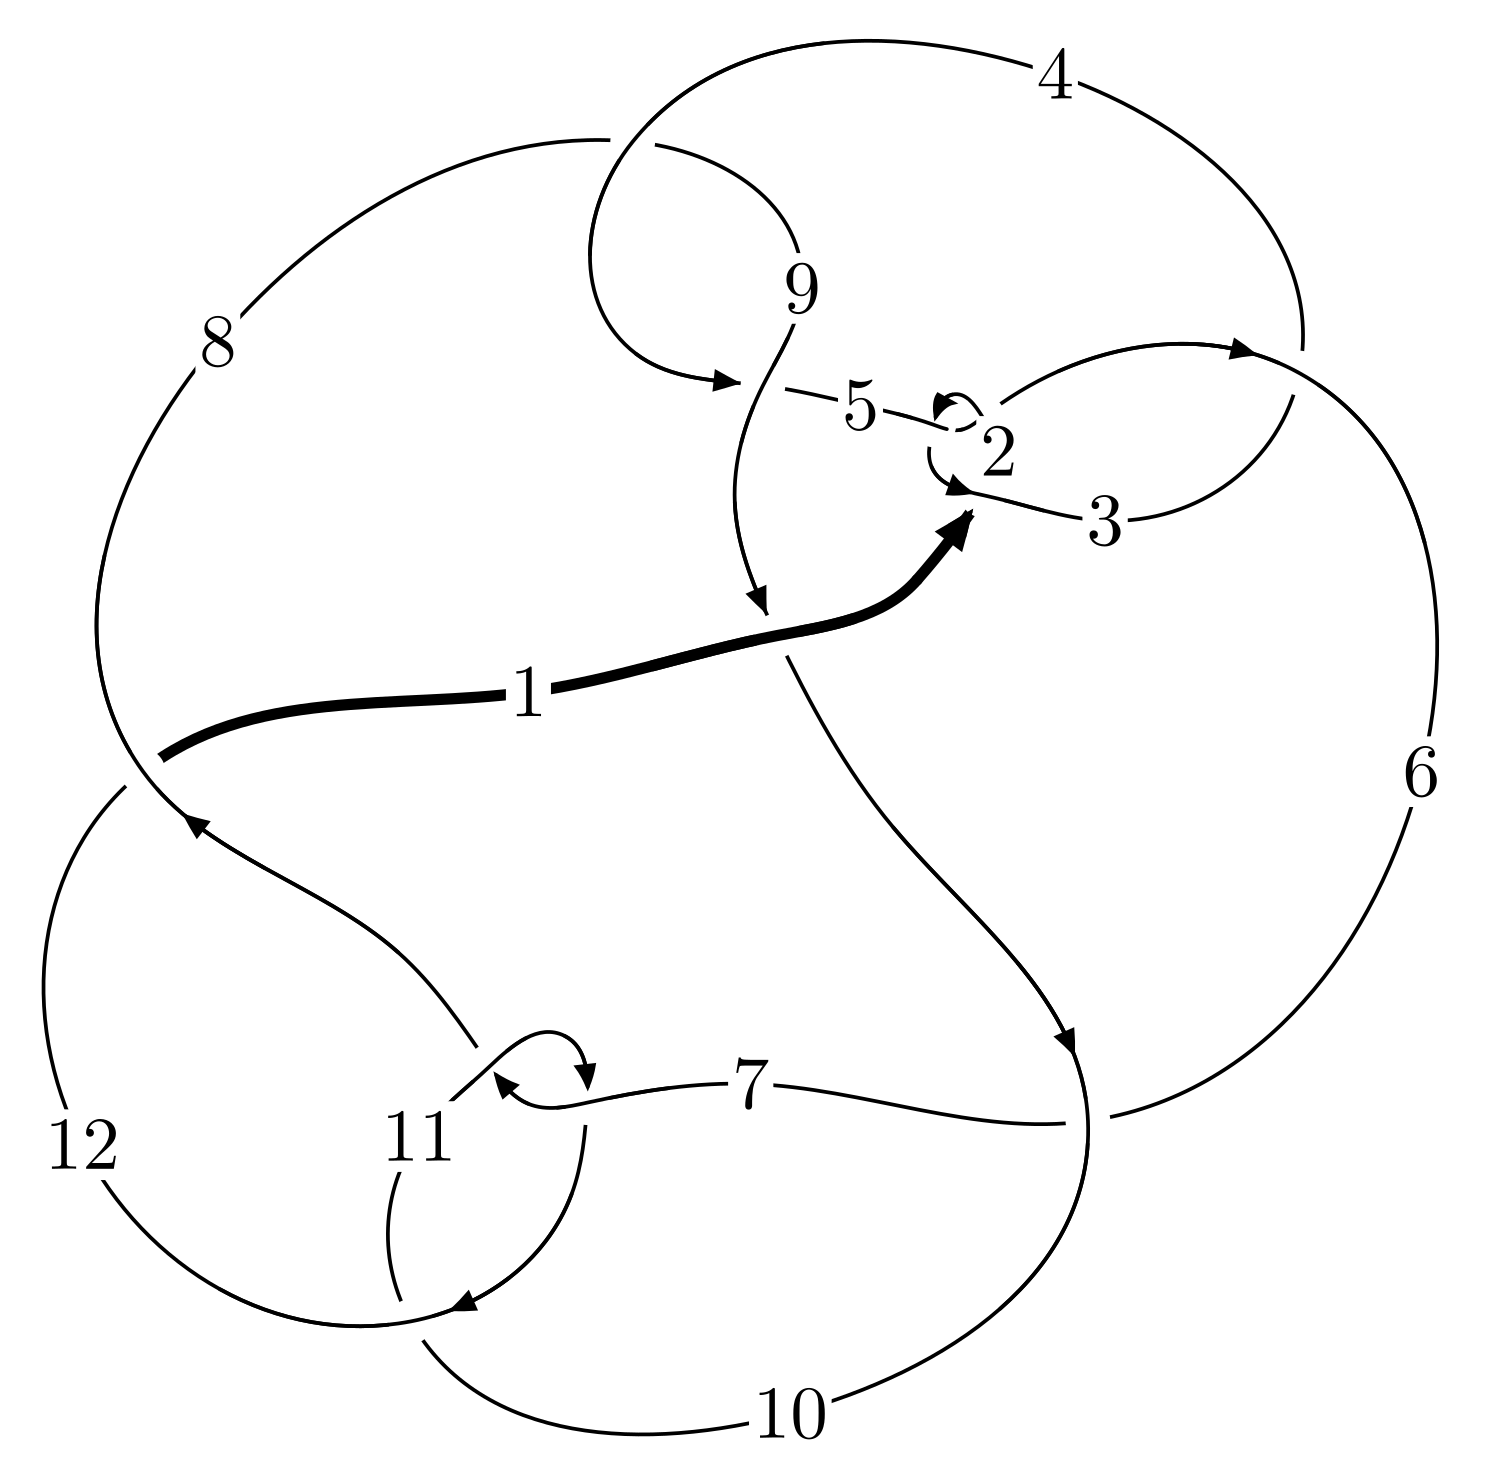
\includegraphics[width=112pt]{../../../GIT/diagram.site/Diagrams/png/817_12a_0016.png}\\
\ \ \ A knot diagram\footnotemark}&
\allowdisplaybreaks
\textbf{Linearized knot diagam} \\
\cline{2-2}
 &
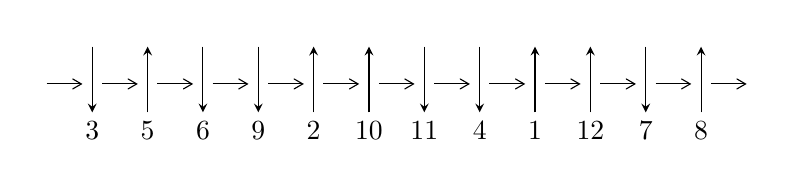
\begin{tikzpicture}[x=20pt, y=17pt]
	% nodes
	\node (C0) at (0, 0) {};
	\node (C1) at (1, 0) {};
	\node (C1U) at (1, +1) {};
	\node (C1D) at (1, -1) {3};

	\node (C2) at (2, 0) {};
	\node (C2U) at (2, +1) {};
	\node (C2D) at (2, -1) {5};

	\node (C3) at (3, 0) {};
	\node (C3U) at (3, +1) {};
	\node (C3D) at (3, -1) {6};

	\node (C4) at (4, 0) {};
	\node (C4U) at (4, +1) {};
	\node (C4D) at (4, -1) {9};

	\node (C5) at (5, 0) {};
	\node (C5U) at (5, +1) {};
	\node (C5D) at (5, -1) {2};

	\node (C6) at (6, 0) {};
	\node (C6U) at (6, +1) {};
	\node (C6D) at (6, -1) {10};

	\node (C7) at (7, 0) {};
	\node (C7U) at (7, +1) {};
	\node (C7D) at (7, -1) {11};

	\node (C8) at (8, 0) {};
	\node (C8U) at (8, +1) {};
	\node (C8D) at (8, -1) {4};

	\node (C9) at (9, 0) {};
	\node (C9U) at (9, +1) {};
	\node (C9D) at (9, -1) {1};

	\node (C10) at (10, 0) {};
	\node (C10U) at (10, +1) {};
	\node (C10D) at (10, -1) {12};

	\node (C11) at (11, 0) {};
	\node (C11U) at (11, +1) {};
	\node (C11D) at (11, -1) {7};

	\node (C12) at (12, 0) {};
	\node (C12U) at (12, +1) {};
	\node (C12D) at (12, -1) {8};
	\node (C13) at (13, 0) {};

	% arrows
	\draw[->,>={angle 60}]
	(C0) edge (C1) (C1) edge (C2) (C2) edge (C3) (C3) edge (C4) (C4) edge (C5) (C5) edge (C6) (C6) edge (C7) (C7) edge (C8) (C8) edge (C9) (C9) edge (C10) (C10) edge (C11) (C11) edge (C12) (C12) edge (C13) ;	\draw[->,>=stealth]
	(C1U) edge (C1D) (C2D) edge (C2U) (C3U) edge (C3D) (C4U) edge (C4D) (C5D) edge (C5U) (C6D) edge (C6U) (C7U) edge (C7D) (C8U) edge (C8D) (C9D) edge (C9U) (C10D) edge (C10U) (C11U) edge (C11D) (C12D) edge (C12U) ;
	\end{tikzpicture} \\
\hhline{~~} \\& 
\textbf{Solving Sequence} \\ \cline{2-2} 
 &
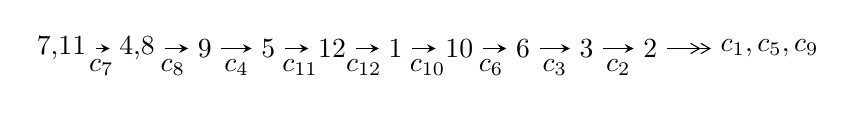
\begin{tikzpicture}[x=23pt, y=7pt]
	% node
	\node (A0) at (-1/8, 0) {7,11};
	\node (A1) at (17/16, 0) {4,8};
	\node (A2) at (17/8, 0) {9};
	\node (A3) at (25/8, 0) {5};
	\node (A4) at (33/8, 0) {12};
	\node (A5) at (41/8, 0) {1};
	\node (A6) at (49/8, 0) {10};
	\node (A7) at (57/8, 0) {6};
	\node (A8) at (65/8, 0) {3};
	\node (A9) at (73/8, 0) {2};
	\node (C1) at (1/2, -1) {$c_{7}$};
	\node (C2) at (13/8, -1) {$c_{8}$};
	\node (C3) at (21/8, -1) {$c_{4}$};
	\node (C4) at (29/8, -1) {$c_{11}$};
	\node (C5) at (37/8, -1) {$c_{12}$};
	\node (C6) at (45/8, -1) {$c_{10}$};
	\node (C7) at (53/8, -1) {$c_{6}$};
	\node (C8) at (61/8, -1) {$c_{3}$};
	\node (C9) at (69/8, -1) {$c_{2}$};
	\node (A10) at (11, 0) {$c_{1},c_{5},c_{9}$};

	% edge
	\draw[->,>=stealth]	
	(A0) edge (A1) (A1) edge (A2) (A2) edge (A3) (A3) edge (A4) (A4) edge (A5) (A5) edge (A6) (A6) edge (A7) (A7) edge (A8) (A8) edge (A9) ;
	\draw[->>,>={angle 60}]	
	(A9) edge (A10);
\end{tikzpicture} \\ 

\end{tabular} \\

\footnotetext{
The image of knot diagram is generated by the software ``\textbf{Draw programme}" developed by Andrew Bartholomew(\url{http://www.layer8.co.uk/maths/draw/index.htm\#Running-draw}), where we modified some parts for our purpose(\url{https://github.com/CATsTAILs/LinksPainter}).
}\phantom \\ \newline 
\centering \textbf{Ideals for irreducible components\footnotemark of $X_{\text{par}}$} 
 
\begin{align*}
I^u_{1}&=\langle 
8 u^{109}-22 u^{108}+\cdots+2 b+6 u,\;-8 u^{109}+24 u^{108}+\cdots+2 a+11,\;u^{110}-3 u^{109}+\cdots-2 u+1\rangle \\
I^u_{2}&=\langle 
- u^2 a+b,\;u^4- u^2 a+2 u^3+a^2- a u+3 u^2- a+2 u+1,\;u^5+u^4+2 u^3+u^2+u+1\rangle \\
\\
\end{align*}
\raggedright * 2 irreducible components of $\dim_{\mathbb{C}}=0$, with total 120 representations.\\
\footnotetext{All coefficients of polynomials are rational numbers. But the coefficients are sometimes approximated in decimal forms when there is not enough margin.}
\newpage
\renewcommand{\arraystretch}{1}
\centering \section*{I. $I^u_{1}= \langle 8 u^{109}-22 u^{108}+\cdots+2 b+6 u,\;-8 u^{109}+24 u^{108}+\cdots+2 a+11,\;u^{110}-3 u^{109}+\cdots-2 u+1 \rangle$}
\flushleft \textbf{(i) Arc colorings}\\
\begin{tabular}{m{7pt} m{180pt} m{7pt} m{180pt} }
\flushright $a_{7}=$&$\begin{pmatrix}1\\0\end{pmatrix}$ \\
\flushright $a_{11}=$&$\begin{pmatrix}0\\u\end{pmatrix}$ \\
\flushright $a_{4}=$&$\begin{pmatrix}4 u^{109}-12 u^{108}+\cdots+\frac{15}{2} u-\frac{11}{2}\\-4 u^{109}+11 u^{108}+\cdots-\frac{1}{2} u^2-3 u\end{pmatrix}$ \\
\flushright $a_{8}=$&$\begin{pmatrix}1\\u^2\end{pmatrix}$ \\
\flushright $a_{9}=$&$\begin{pmatrix}- u^{11}-2 u^9-2 u^7- u^3\\- u^{13}-3 u^{11}-5 u^9-4 u^7-2 u^5+u^3+u\end{pmatrix}$ \\
\flushright $a_{5}=$&$\begin{pmatrix}4 u^{108}-8 u^{107}+\cdots-\frac{3}{2} u+\frac{1}{2}\\-2 u^{108}+\frac{5}{2} u^{107}+\cdots-\frac{11}{2} u^2+3 u\end{pmatrix}$ \\
\flushright $a_{12}=$&$\begin{pmatrix}- u\\u\end{pmatrix}$ \\
\flushright $a_{1}=$&$\begin{pmatrix}u^3\\u^5+u^3+u\end{pmatrix}$ \\
\flushright $a_{10}=$&$\begin{pmatrix}- u^3\\u^3+u\end{pmatrix}$ \\
\flushright $a_{6}=$&$\begin{pmatrix}- u^6- u^4+1\\u^6+2 u^4+u^2\end{pmatrix}$ \\
\flushright $a_{3}=$&$\begin{pmatrix}2 u^{109}-\frac{11}{2} u^{108}+\cdots+6 u-3\\-2 u^{109}+\frac{11}{2} u^{108}+\cdots-\frac{3}{2} u^2-\frac{1}{2} u\end{pmatrix}$ \\
\flushright $a_{2}=$&$\begin{pmatrix}-\frac{1}{2} u^{108}+u^{107}+\cdots+2 u-1\\\frac{1}{2} u^{108}- u^{107}+\cdots-\frac{3}{2} u^2+\frac{3}{2} u\end{pmatrix}$\\&\end{tabular}
\flushleft \textbf{(ii) Obstruction class $= -1$}\\~\\
\flushleft \textbf{(iii) Cusp Shapes $= 4 u^{109}-\frac{31}{2} u^{108}+\cdots+\frac{47}{2} u-\frac{15}{2}$}\\~\\
\newpage\renewcommand{\arraystretch}{1}
\flushleft \textbf{(iv) u-Polynomials at the component}\newline \\
\begin{tabular}{m{50pt}|m{274pt}}
Crossings & \hspace{64pt}u-Polynomials at each crossing \\
\hline $$\begin{aligned}c_{1}\end{aligned}$$&$\begin{aligned}
&u^{110}+54 u^{109}+\cdots+7 u+1
\end{aligned}$\\
\hline $$\begin{aligned}c_{2},c_{5}\end{aligned}$$&$\begin{aligned}
&u^{110}+6 u^{109}+\cdots+5 u+1
\end{aligned}$\\
\hline $$\begin{aligned}c_{3}\end{aligned}$$&$\begin{aligned}
&u^{110}-6 u^{109}+\cdots-455049 u+73746
\end{aligned}$\\
\hline $$\begin{aligned}c_{4},c_{8}\end{aligned}$$&$\begin{aligned}
&u^{110}- u^{109}+\cdots-10240 u^2+1024
\end{aligned}$\\
\hline $$\begin{aligned}c_{6},c_{12}\end{aligned}$$&$\begin{aligned}
&u^{110}-3 u^{109}+\cdots-585 u+34
\end{aligned}$\\
\hline $$\begin{aligned}c_{7},c_{11}\end{aligned}$$&$\begin{aligned}
&u^{110}+3 u^{109}+\cdots+2 u+1
\end{aligned}$\\
\hline $$\begin{aligned}c_{9}\end{aligned}$$&$\begin{aligned}
&u^{110}+13 u^{109}+\cdots+74128 u+1669
\end{aligned}$\\
\hline $$\begin{aligned}c_{10}\end{aligned}$$&$\begin{aligned}
&u^{110}-59 u^{109}+\cdots-8 u+1
\end{aligned}$\\
\hline
\end{tabular}\\~\\
\newpage\renewcommand{\arraystretch}{1}
\flushleft \textbf{(v) Riley Polynomials at the component}\newline \\
\begin{tabular}{m{50pt}|m{274pt}}
Crossings & \hspace{64pt}Riley Polynomials at each crossing \\
\hline $$\begin{aligned}c_{1}\end{aligned}$$&$\begin{aligned}
&y^{110}+10 y^{109}+\cdots-9 y+1
\end{aligned}$\\
\hline $$\begin{aligned}c_{2},c_{5}\end{aligned}$$&$\begin{aligned}
&y^{110}+54 y^{109}+\cdots+7 y+1
\end{aligned}$\\
\hline $$\begin{aligned}c_{3}\end{aligned}$$&$\begin{aligned}
&y^{110}-34 y^{109}+\cdots-23865354441 y+5438472516
\end{aligned}$\\
\hline $$\begin{aligned}c_{4},c_{8}\end{aligned}$$&$\begin{aligned}
&y^{110}-55 y^{109}+\cdots-20971520 y+1048576
\end{aligned}$\\
\hline $$\begin{aligned}c_{6},c_{12}\end{aligned}$$&$\begin{aligned}
&y^{110}-85 y^{109}+\cdots+105147 y+1156
\end{aligned}$\\
\hline $$\begin{aligned}c_{7},c_{11}\end{aligned}$$&$\begin{aligned}
&y^{110}+59 y^{109}+\cdots+8 y+1
\end{aligned}$\\
\hline $$\begin{aligned}c_{9}\end{aligned}$$&$\begin{aligned}
&y^{110}+15 y^{109}+\cdots-1624602792 y+2785561
\end{aligned}$\\
\hline $$\begin{aligned}c_{10}\end{aligned}$$&$\begin{aligned}
&y^{110}-13 y^{109}+\cdots+76 y+1
\end{aligned}$\\
\hline
\end{tabular}\\~\\
\newpage\flushleft \textbf{(vi) Complex Volumes and Cusp Shapes}
$$\begin{array}{c|c|c}  
\text{Solutions to }I^u_{1}& \I (\text{vol} + \sqrt{-1}CS) & \text{Cusp shape}\\
 \hline 
\begin{aligned}
u &= -0.579982 + 0.823482 I \\
a &= -1.10813 - 1.57808 I \\
b &= \phantom{-}0.196290 + 1.248310 I\end{aligned}
 & -7.69991 + 3.23271 I & \phantom{-0.000000 } 0 \\ \hline\begin{aligned}
u &= -0.579982 - 0.823482 I \\
a &= -1.10813 + 1.57808 I \\
b &= \phantom{-}0.196290 - 1.248310 I\end{aligned}
 & -7.69991 - 3.23271 I & \phantom{-0.000000 } 0 \\ \hline\begin{aligned}
u &= -0.561599 + 0.852113 I \\
a &= \phantom{-}1.26319 + 1.80130 I \\
b &= \phantom{-}0.00553 - 1.44932 I\end{aligned}
 & -3.12530 + 6.60837 I & \phantom{-0.000000 } 0 \\ \hline\begin{aligned}
u &= -0.561599 - 0.852113 I \\
a &= \phantom{-}1.26319 - 1.80130 I \\
b &= \phantom{-}0.00553 + 1.44932 I\end{aligned}
 & -3.12530 - 6.60837 I & \phantom{-0.000000 } 0 \\ \hline\begin{aligned}
u &= \phantom{-}0.406550 + 0.888189 I \\
a &= -0.690850 - 0.195917 I \\
b &= \phantom{-}0.0799002 + 0.0496905 I\end{aligned}
 & \phantom{-}0.19398 - 2.02003 I & \phantom{-0.000000 } 0 \\ \hline\begin{aligned}
u &= \phantom{-}0.406550 - 0.888189 I \\
a &= -0.690850 + 0.195917 I \\
b &= \phantom{-}0.0799002 - 0.0496905 I\end{aligned}
 & \phantom{-}0.19398 + 2.02003 I & \phantom{-0.000000 } 0 \\ \hline\begin{aligned}
u &= \phantom{-}0.528135 + 0.808914 I \\
a &= \phantom{-}1.011690 - 0.239556 I \\
b &= \phantom{-}0.0721671 - 0.1011930 I\end{aligned}
 & -2.50066 - 5.75747 I & \phantom{-0.000000 } 0 \\ \hline\begin{aligned}
u &= \phantom{-}0.528135 - 0.808914 I \\
a &= \phantom{-}1.011690 + 0.239556 I \\
b &= \phantom{-}0.0721671 + 0.1011930 I\end{aligned}
 & -2.50066 + 5.75747 I & \phantom{-0.000000 } 0 \\ \hline\begin{aligned}
u &= -0.577603 + 0.864674 I \\
a &= -1.14476 - 1.89716 I \\
b &= -0.142767 + 1.339650 I\end{aligned}
 & -5.80226 + 11.67560 I & \phantom{-0.000000 } 0 \\ \hline\begin{aligned}
u &= -0.577603 - 0.864674 I \\
a &= -1.14476 + 1.89716 I \\
b &= -0.142767 - 1.339650 I\end{aligned}
 & -5.80226 - 11.67560 I & \phantom{-0.000000 } 0\\
 \hline 
 \end{array}$$\newpage$$\begin{array}{c|c|c}  
\text{Solutions to }I^u_{1}& \I (\text{vol} + \sqrt{-1}CS) & \text{Cusp shape}\\
 \hline 
\begin{aligned}
u &= \phantom{-}0.128950 + 1.034770 I \\
a &= -1.07011 - 1.42517 I \\
b &= \phantom{-}0.553854 + 0.773753 I\end{aligned}
 & \phantom{-}1.55547 - 2.74435 I & \phantom{-0.000000 } 0 \\ \hline\begin{aligned}
u &= \phantom{-}0.128950 - 1.034770 I \\
a &= -1.07011 + 1.42517 I \\
b &= \phantom{-}0.553854 - 0.773753 I\end{aligned}
 & \phantom{-}1.55547 + 2.74435 I & \phantom{-0.000000 } 0 \\ \hline\begin{aligned}
u &= -0.487300 + 0.806990 I \\
a &= \phantom{-}1.99235 + 1.41659 I \\
b &= -0.57504 - 1.94110 I\end{aligned}
 & -0.42932 + 4.54389 I & \phantom{-0.000000 } 0 \\ \hline\begin{aligned}
u &= -0.487300 - 0.806990 I \\
a &= \phantom{-}1.99235 - 1.41659 I \\
b &= -0.57504 + 1.94110 I\end{aligned}
 & -0.42932 - 4.54389 I & \phantom{-0.000000 } 0 \\ \hline\begin{aligned}
u &= \phantom{-}0.011304 + 0.929219 I \\
a &= -0.35995 - 1.94849 I \\
b &= -0.263245 + 1.087660 I\end{aligned}
 & \phantom{-}2.57030 - 1.41361 I & \phantom{-0.000000 } 0 \\ \hline\begin{aligned}
u &= \phantom{-}0.011304 - 0.929219 I \\
a &= -0.35995 + 1.94849 I \\
b &= -0.263245 - 1.087660 I\end{aligned}
 & \phantom{-}2.57030 + 1.41361 I & \phantom{-0.000000 } 0 \\ \hline\begin{aligned}
u &= -0.592873 + 0.707362 I \\
a &= \phantom{-}0.861643 + 0.645026 I \\
b &= -0.91828 - 1.09414 I\end{aligned}
 & -8.03143 + 1.39305 I & \phantom{-0.000000 } 0 \\ \hline\begin{aligned}
u &= -0.592873 - 0.707362 I \\
a &= \phantom{-}0.861643 - 0.645026 I \\
b &= -0.91828 + 1.09414 I\end{aligned}
 & -8.03143 - 1.39305 I & \phantom{-0.000000 } 0 \\ \hline\begin{aligned}
u &= \phantom{-}0.452920 + 0.800781 I \\
a &= -0.763988 + 0.178725 I \\
b &= \phantom{-}0.0478287 + 0.0879934 I\end{aligned}
 & -0.04986 - 1.88964 I & \phantom{-0.000000 } 0 \\ \hline\begin{aligned}
u &= \phantom{-}0.452920 - 0.800781 I \\
a &= -0.763988 - 0.178725 I \\
b &= \phantom{-}0.0478287 - 0.0879934 I\end{aligned}
 & -0.04986 + 1.88964 I & \phantom{-0.000000 } 0\\
 \hline 
 \end{array}$$\newpage$$\begin{array}{c|c|c}  
\text{Solutions to }I^u_{1}& \I (\text{vol} + \sqrt{-1}CS) & \text{Cusp shape}\\
 \hline 
\begin{aligned}
u &= \phantom{-}0.128527 + 1.087170 I \\
a &= \phantom{-}1.41312 + 1.45257 I \\
b &= -0.928389 - 0.812896 I\end{aligned}
 & -0.83737 - 7.40305 I & \phantom{-0.000000 } 0 \\ \hline\begin{aligned}
u &= \phantom{-}0.128527 - 1.087170 I \\
a &= \phantom{-}1.41312 - 1.45257 I \\
b &= -0.928389 + 0.812896 I\end{aligned}
 & -0.83737 + 7.40305 I & \phantom{-0.000000 } 0 \\ \hline\begin{aligned}
u &= \phantom{-}0.226104 + 1.082150 I \\
a &= \phantom{-}1.30997 + 0.79217 I \\
b &= -0.731357 - 0.110538 I\end{aligned}
 & -2.18609 + 0.20029 I & \phantom{-0.000000 } 0 \\ \hline\begin{aligned}
u &= \phantom{-}0.226104 - 1.082150 I \\
a &= \phantom{-}1.30997 - 0.79217 I \\
b &= -0.731357 + 0.110538 I\end{aligned}
 & -2.18609 - 0.20029 I & \phantom{-0.000000 } 0 \\ \hline\begin{aligned}
u &= \phantom{-}0.521951 + 0.724522 I \\
a &= \phantom{-}0.874689 - 0.434640 I \\
b &= -0.029472 - 0.261786 I\end{aligned}
 & -2.74492 + 1.47945 I & \phantom{-0.000000 } 0 \\ \hline\begin{aligned}
u &= \phantom{-}0.521951 - 0.724522 I \\
a &= \phantom{-}0.874689 + 0.434640 I \\
b &= -0.029472 + 0.261786 I\end{aligned}
 & -2.74492 - 1.47945 I & \phantom{-0.000000 } 0 \\ \hline\begin{aligned}
u &= -0.603428 + 0.653495 I \\
a &= \phantom{-}0.705508 + 0.281490 I \\
b &= -1.10269 - 1.10590 I\end{aligned}
 & -6.40282 - 7.03071 I & \phantom{-0.000000 } 0 \\ \hline\begin{aligned}
u &= -0.603428 - 0.653495 I \\
a &= \phantom{-}0.705508 - 0.281490 I \\
b &= -1.10269 + 1.10590 I\end{aligned}
 & -6.40282 + 7.03071 I & \phantom{-0.000000 } 0 \\ \hline\begin{aligned}
u &= -0.087587 + 0.882466 I \\
a &= -0.05146 + 2.36788 I \\
b &= \phantom{-}0.85301 - 1.20943 I\end{aligned}
 & \phantom{-}1.34153 + 3.06537 I & \phantom{-}5.56421 + 0. I\phantom{ +0.000000I} \\ \hline\begin{aligned}
u &= -0.087587 - 0.882466 I \\
a &= -0.05146 - 2.36788 I \\
b &= \phantom{-}0.85301 + 1.20943 I\end{aligned}
 & \phantom{-}1.34153 - 3.06537 I & \phantom{-}5.56421 + 0. I\phantom{ +0.000000I}\\
 \hline 
 \end{array}$$\newpage$$\begin{array}{c|c|c}  
\text{Solutions to }I^u_{1}& \I (\text{vol} + \sqrt{-1}CS) & \text{Cusp shape}\\
 \hline 
\begin{aligned}
u &= -0.467459 + 0.752773 I \\
a &= -2.12256 - 0.69643 I \\
b &= \phantom{-}1.06350 + 1.76434 I\end{aligned}
 & -0.606282 - 0.555086 I & -5.95291 + 0. I\phantom{ +0.000000I} \\ \hline\begin{aligned}
u &= -0.467459 - 0.752773 I \\
a &= -2.12256 + 0.69643 I \\
b &= \phantom{-}1.06350 - 1.76434 I\end{aligned}
 & -0.606282 + 0.555086 I & -5.95291 + 0. I\phantom{ +0.000000I} \\ \hline\begin{aligned}
u &= -0.575057 + 0.665687 I \\
a &= -0.913960 - 0.314089 I \\
b &= \phantom{-}1.05186 + 1.16392 I\end{aligned}
 & -3.65420 - 2.08576 I & \phantom{-0.000000 } 0 \\ \hline\begin{aligned}
u &= -0.575057 - 0.665687 I \\
a &= -0.913960 + 0.314089 I \\
b &= \phantom{-}1.05186 - 1.16392 I\end{aligned}
 & -3.65420 + 2.08576 I & \phantom{-0.000000 } 0 \\ \hline\begin{aligned}
u &= \phantom{-}0.819934 + 0.162919 I \\
a &= -0.41914 - 1.36387 I \\
b &= \phantom{-}1.32289 - 1.67361 I\end{aligned}
 & -2.26724 + 12.52740 I & -2.80434 - 7.99531 I \\ \hline\begin{aligned}
u &= \phantom{-}0.819934 - 0.162919 I \\
a &= -0.41914 + 1.36387 I \\
b &= \phantom{-}1.32289 + 1.67361 I\end{aligned}
 & -2.26724 - 12.52740 I & -2.80434 + 7.99531 I \\ \hline\begin{aligned}
u &= -0.828291 + 0.028957 I \\
a &= \phantom{-}0.701648 - 0.191250 I \\
b &= \phantom{-}1.336090 - 0.429868 I\end{aligned}
 & \phantom{-}1.62988 + 3.17856 I & -3.50751 - 5.52897 I \\ \hline\begin{aligned}
u &= -0.828291 - 0.028957 I \\
a &= \phantom{-}0.701648 + 0.191250 I \\
b &= \phantom{-}1.336090 + 0.429868 I\end{aligned}
 & \phantom{-}1.62988 - 3.17856 I & -3.50751 + 5.52897 I \\ \hline\begin{aligned}
u &= \phantom{-}0.806530 + 0.157966 I \\
a &= \phantom{-}0.53866 + 1.33941 I \\
b &= -1.17343 + 1.59078 I\end{aligned}
 & \phantom{-}0.21834 + 7.31585 I & \phantom{-0.000000 } 0. - 4.55869 I \\ \hline\begin{aligned}
u &= \phantom{-}0.806530 - 0.157966 I \\
a &= \phantom{-}0.53866 - 1.33941 I \\
b &= -1.17343 - 1.59078 I\end{aligned}
 & \phantom{-}0.21834 - 7.31585 I & \phantom{-0.000000 -}0. + 4.55869 I\\
 \hline 
 \end{array}$$\newpage$$\begin{array}{c|c|c}  
\text{Solutions to }I^u_{1}& \I (\text{vol} + \sqrt{-1}CS) & \text{Cusp shape}\\
 \hline 
\begin{aligned}
u &= \phantom{-}0.792107 + 0.182923 I \\
a &= -0.519053 - 1.102450 I \\
b &= \phantom{-}1.27628 - 1.28558 I\end{aligned}
 & -4.65166 + 4.23372 I & -5.98881 - 2.52410 I \\ \hline\begin{aligned}
u &= \phantom{-}0.792107 - 0.182923 I \\
a &= -0.519053 + 1.102450 I \\
b &= \phantom{-}1.27628 + 1.28558 I\end{aligned}
 & -4.65166 - 4.23372 I & -5.98881 + 2.52410 I \\ \hline\begin{aligned}
u &= \phantom{-}0.507208 + 1.073690 I \\
a &= \phantom{-}0.813220 + 1.009570 I \\
b &= -0.554966 - 0.329840 I\end{aligned}
 & -3.13792 + 0.92257 I & \phantom{-0.000000 } 0 \\ \hline\begin{aligned}
u &= \phantom{-}0.507208 - 1.073690 I \\
a &= \phantom{-}0.813220 - 1.009570 I \\
b &= -0.554966 + 0.329840 I\end{aligned}
 & -3.13792 - 0.92257 I & \phantom{-0.000000 } 0 \\ \hline\begin{aligned}
u &= -0.795193 + 0.053029 I \\
a &= -0.528875 + 0.373665 I \\
b &= -0.905963 + 0.770490 I\end{aligned}
 & \phantom{-}3.25367 - 0.82072 I & \phantom{-}2.37894 - 1.72031 I \\ \hline\begin{aligned}
u &= -0.795193 - 0.053029 I \\
a &= -0.528875 - 0.373665 I \\
b &= -0.905963 - 0.770490 I\end{aligned}
 & \phantom{-}3.25367 + 0.82072 I & \phantom{-}2.37894 + 1.72031 I \\ \hline\begin{aligned}
u &= \phantom{-}0.488937 + 1.104850 I \\
a &= -0.432111 - 1.066750 I \\
b &= \phantom{-}0.387961 + 0.735312 I\end{aligned}
 & -0.04787 - 3.54238 I & \phantom{-0.000000 } 0 \\ \hline\begin{aligned}
u &= \phantom{-}0.488937 - 1.104850 I \\
a &= -0.432111 + 1.066750 I \\
b &= \phantom{-}0.387961 - 0.735312 I\end{aligned}
 & -0.04787 + 3.54238 I & \phantom{-0.000000 } 0 \\ \hline\begin{aligned}
u &= -0.767663 + 0.149617 I \\
a &= \phantom{-}0.522352 - 0.771363 I \\
b &= \phantom{-}0.54928 - 1.61345 I\end{aligned}
 & \phantom{-}0.28498 - 6.22966 I & -1.67005 + 5.40696 I \\ \hline\begin{aligned}
u &= -0.767663 - 0.149617 I \\
a &= \phantom{-}0.522352 + 0.771363 I \\
b &= \phantom{-}0.54928 + 1.61345 I\end{aligned}
 & \phantom{-}0.28498 + 6.22966 I & -1.67005 - 5.40696 I\\
 \hline 
 \end{array}$$\newpage$$\begin{array}{c|c|c}  
\text{Solutions to }I^u_{1}& \I (\text{vol} + \sqrt{-1}CS) & \text{Cusp shape}\\
 \hline 
\begin{aligned}
u &= -0.413961 + 1.146140 I \\
a &= \phantom{-}0.43422 + 2.07516 I \\
b &= \phantom{-}1.20426 - 1.84563 I\end{aligned}
 & \phantom{-}2.54580 + 4.57308 I & \phantom{-0.000000 } 0 \\ \hline\begin{aligned}
u &= -0.413961 - 1.146140 I \\
a &= \phantom{-}0.43422 - 2.07516 I \\
b &= \phantom{-}1.20426 + 1.84563 I\end{aligned}
 & \phantom{-}2.54580 - 4.57308 I & \phantom{-0.000000 } 0 \\ \hline\begin{aligned}
u &= \phantom{-}0.763221 + 0.125905 I \\
a &= \phantom{-}1.04676 + 1.31046 I \\
b &= -0.59709 + 1.37823 I\end{aligned}
 & \phantom{-}2.27168 + 4.64244 I & \phantom{-}0.14088 - 6.23456 I \\ \hline\begin{aligned}
u &= \phantom{-}0.763221 - 0.125905 I \\
a &= \phantom{-}1.04676 - 1.31046 I \\
b &= -0.59709 - 1.37823 I\end{aligned}
 & \phantom{-}2.27168 - 4.64244 I & \phantom{-}0.14088 + 6.23456 I \\ \hline\begin{aligned}
u &= -0.759138 + 0.112943 I \\
a &= -0.473360 + 0.674125 I \\
b &= -0.57188 + 1.33475 I\end{aligned}
 & \phantom{-}2.55409 - 1.75029 I & \phantom{-}2.58514 + 1.16963 I \\ \hline\begin{aligned}
u &= -0.759138 - 0.112943 I \\
a &= -0.473360 - 0.674125 I \\
b &= -0.57188 - 1.33475 I\end{aligned}
 & \phantom{-}2.55409 + 1.75029 I & \phantom{-}2.58514 - 1.16963 I \\ \hline\begin{aligned}
u &= \phantom{-}0.517547 + 1.118880 I \\
a &= \phantom{-}0.54435 + 1.49296 I \\
b &= -0.917306 - 0.885875 I\end{aligned}
 & -3.84920 - 7.45703 I & \phantom{-0.000000 } 0 \\ \hline\begin{aligned}
u &= \phantom{-}0.517547 - 1.118880 I \\
a &= \phantom{-}0.54435 - 1.49296 I \\
b &= -0.917306 + 0.885875 I\end{aligned}
 & -3.84920 + 7.45703 I & \phantom{-0.000000 } 0 \\ \hline\begin{aligned}
u &= \phantom{-}0.348172 + 1.192970 I \\
a &= -1.31970 + 0.77788 I \\
b &= -0.12251 - 1.61626 I\end{aligned}
 & -0.502173 + 0.513562 I & \phantom{-0.000000 } 0 \\ \hline\begin{aligned}
u &= \phantom{-}0.348172 - 1.192970 I \\
a &= -1.31970 - 0.77788 I \\
b &= -0.12251 + 1.61626 I\end{aligned}
 & -0.502173 - 0.513562 I & \phantom{-0.000000 } 0\\
 \hline 
 \end{array}$$\newpage$$\begin{array}{c|c|c}  
\text{Solutions to }I^u_{1}& \I (\text{vol} + \sqrt{-1}CS) & \text{Cusp shape}\\
 \hline 
\begin{aligned}
u &= -0.379263 + 1.186000 I \\
a &= -0.16882 + 2.36666 I \\
b &= \phantom{-}1.84998 - 1.82441 I\end{aligned}
 & \phantom{-}4.19584 - 2.40976 I & \phantom{-0.000000 } 0 \\ \hline\begin{aligned}
u &= -0.379263 - 1.186000 I \\
a &= -0.16882 - 2.36666 I \\
b &= \phantom{-}1.84998 + 1.82441 I\end{aligned}
 & \phantom{-}4.19584 + 2.40976 I & \phantom{-0.000000 } 0 \\ \hline\begin{aligned}
u &= \phantom{-}0.698012 + 0.281638 I \\
a &= \phantom{-}0.607096 + 0.269495 I \\
b &= -1.162940 + 0.229128 I\end{aligned}
 & -6.27859 + 2.81930 I & -7.65388 - 2.76519 I \\ \hline\begin{aligned}
u &= \phantom{-}0.698012 - 0.281638 I \\
a &= \phantom{-}0.607096 - 0.269495 I \\
b &= -1.162940 - 0.229128 I\end{aligned}
 & -6.27859 - 2.81930 I & -7.65388 + 2.76519 I \\ \hline\begin{aligned}
u &= \phantom{-}0.407392 + 1.179060 I \\
a &= -0.068976 + 0.937001 I \\
b &= -1.67160 - 0.80250 I\end{aligned}
 & \phantom{-}5.23948 - 4.51130 I & \phantom{-0.000000 } 0 \\ \hline\begin{aligned}
u &= \phantom{-}0.407392 - 1.179060 I \\
a &= -0.068976 - 0.937001 I \\
b &= -1.67160 + 0.80250 I\end{aligned}
 & \phantom{-}5.23948 + 4.51130 I & \phantom{-0.000000 } 0 \\ \hline\begin{aligned}
u &= \phantom{-}0.392928 + 1.189590 I \\
a &= \phantom{-}0.510361 - 1.133510 I \\
b &= \phantom{-}1.34113 + 1.39839 I\end{aligned}
 & \phantom{-}6.09922 + 0.72292 I & \phantom{-0.000000 } 0 \\ \hline\begin{aligned}
u &= \phantom{-}0.392928 - 1.189590 I \\
a &= \phantom{-}0.510361 + 1.133510 I \\
b &= \phantom{-}1.34113 - 1.39839 I\end{aligned}
 & \phantom{-}6.09922 - 0.72292 I & \phantom{-0.000000 } 0 \\ \hline\begin{aligned}
u &= \phantom{-}0.657190 + 0.353180 I \\
a &= \phantom{-}0.603599 - 0.062740 I \\
b &= -1.035640 - 0.145534 I\end{aligned}
 & -5.21588 - 5.43372 I & -6.35737 + 4.53160 I \\ \hline\begin{aligned}
u &= \phantom{-}0.657190 - 0.353180 I \\
a &= \phantom{-}0.603599 + 0.062740 I \\
b &= -1.035640 + 0.145534 I\end{aligned}
 & -5.21588 + 5.43372 I & -6.35737 - 4.53160 I\\
 \hline 
 \end{array}$$\newpage$$\begin{array}{c|c|c}  
\text{Solutions to }I^u_{1}& \I (\text{vol} + \sqrt{-1}CS) & \text{Cusp shape}\\
 \hline 
\begin{aligned}
u &= -0.399775 + 1.189730 I \\
a &= \phantom{-}0.21805 - 2.06307 I \\
b &= -1.73761 + 1.50516 I\end{aligned}
 & \phantom{-}6.33069 + 2.21234 I & \phantom{-0.000000 } 0 \\ \hline\begin{aligned}
u &= -0.399775 - 1.189730 I \\
a &= \phantom{-}0.21805 + 2.06307 I \\
b &= -1.73761 - 1.50516 I\end{aligned}
 & \phantom{-}6.33069 - 2.21234 I & \phantom{-0.000000 } 0 \\ \hline\begin{aligned}
u &= -0.491061 + 1.156340 I \\
a &= -1.35904 - 1.51080 I \\
b &= -0.38225 + 2.14323 I\end{aligned}
 & \phantom{-}1.97040 + 3.53194 I & \phantom{-0.000000 } 0 \\ \hline\begin{aligned}
u &= -0.491061 - 1.156340 I \\
a &= -1.35904 + 1.51080 I \\
b &= -0.38225 - 2.14323 I\end{aligned}
 & \phantom{-}1.97040 - 3.53194 I & \phantom{-0.000000 } 0 \\ \hline\begin{aligned}
u &= \phantom{-}0.732239 + 0.108513 I \\
a &= -1.38411 - 1.13292 I \\
b &= \phantom{-}0.307181 - 1.116300 I\end{aligned}
 & \phantom{-}1.58615 - 0.58965 I & -2.07800 - 0.97177 I \\ \hline\begin{aligned}
u &= \phantom{-}0.732239 - 0.108513 I \\
a &= -1.38411 + 1.13292 I \\
b &= \phantom{-}0.307181 + 1.116300 I\end{aligned}
 & \phantom{-}1.58615 + 0.58965 I & -2.07800 + 0.97177 I \\ \hline\begin{aligned}
u &= \phantom{-}0.365257 + 1.209930 I \\
a &= \phantom{-}1.26314 - 1.20974 I \\
b &= \phantom{-}0.51622 + 2.09356 I\end{aligned}
 & \phantom{-}4.34795 + 3.40901 I & \phantom{-0.000000 } 0 \\ \hline\begin{aligned}
u &= \phantom{-}0.365257 - 1.209930 I \\
a &= \phantom{-}1.26314 + 1.20974 I \\
b &= \phantom{-}0.51622 - 2.09356 I\end{aligned}
 & \phantom{-}4.34795 - 3.40901 I & \phantom{-0.000000 } 0 \\ \hline\begin{aligned}
u &= \phantom{-}0.359487 + 1.219040 I \\
a &= -1.46794 + 1.26755 I \\
b &= -0.30978 - 2.32417 I\end{aligned}
 & \phantom{-}1.94636 + 8.59411 I & \phantom{-0.000000 } 0 \\ \hline\begin{aligned}
u &= \phantom{-}0.359487 - 1.219040 I \\
a &= -1.46794 - 1.26755 I \\
b &= -0.30978 + 2.32417 I\end{aligned}
 & \phantom{-}1.94636 - 8.59411 I & \phantom{-0.000000 } 0\\
 \hline 
 \end{array}$$\newpage$$\begin{array}{c|c|c}  
\text{Solutions to }I^u_{1}& \I (\text{vol} + \sqrt{-1}CS) & \text{Cusp shape}\\
 \hline 
\begin{aligned}
u &= \phantom{-}0.490134 + 1.175270 I \\
a &= \phantom{-}0.75303 - 2.05112 I \\
b &= \phantom{-}0.57013 + 2.89728 I\end{aligned}
 & \phantom{-}4.64951 - 3.96013 I & \phantom{-0.000000 } 0 \\ \hline\begin{aligned}
u &= \phantom{-}0.490134 - 1.175270 I \\
a &= \phantom{-}0.75303 + 2.05112 I \\
b &= \phantom{-}0.57013 - 2.89728 I\end{aligned}
 & \phantom{-}4.64951 + 3.96013 I & \phantom{-0.000000 } 0 \\ \hline\begin{aligned}
u &= -0.494920 + 1.182490 I \\
a &= \phantom{-}1.55048 + 1.06172 I \\
b &= -0.12686 - 2.10588 I\end{aligned}
 & \phantom{-}5.65654 + 6.38567 I & \phantom{-0.000000 } 0 \\ \hline\begin{aligned}
u &= -0.494920 - 1.182490 I \\
a &= \phantom{-}1.55048 - 1.06172 I \\
b &= -0.12686 + 2.10588 I\end{aligned}
 & \phantom{-}5.65654 - 6.38567 I & \phantom{-0.000000 } 0 \\ \hline\begin{aligned}
u &= \phantom{-}0.499816 + 1.182010 I \\
a &= -0.56993 + 2.39465 I \\
b &= -1.18433 - 2.97646 I\end{aligned}
 & \phantom{-}5.34282 - 9.31716 I & \phantom{-0.000000 } 0 \\ \hline\begin{aligned}
u &= \phantom{-}0.499816 - 1.182010 I \\
a &= -0.56993 - 2.39465 I \\
b &= -1.18433 + 2.97646 I\end{aligned}
 & \phantom{-}5.34282 + 9.31716 I & \phantom{-0.000000 } 0 \\ \hline\begin{aligned}
u &= -0.507954 + 1.179230 I \\
a &= -1.76230 - 1.22811 I \\
b &= \phantom{-}0.06729 + 2.40466 I\end{aligned}
 & \phantom{-}3.28961 + 10.96240 I & \phantom{-0.000000 } 0 \\ \hline\begin{aligned}
u &= -0.507954 - 1.179230 I \\
a &= -1.76230 + 1.22811 I \\
b &= \phantom{-}0.06729 - 2.40466 I\end{aligned}
 & \phantom{-}3.28961 - 10.96240 I & \phantom{-0.000000 } 0 \\ \hline\begin{aligned}
u &= -0.428422 + 1.211720 I \\
a &= \phantom{-}0.67472 - 1.44248 I \\
b &= -1.73574 + 0.61936 I\end{aligned}
 & \phantom{-}6.98159 + 3.47872 I & \phantom{-0.000000 } 0 \\ \hline\begin{aligned}
u &= -0.428422 - 1.211720 I \\
a &= \phantom{-}0.67472 + 1.44248 I \\
b &= -1.73574 - 0.61936 I\end{aligned}
 & \phantom{-}6.98159 - 3.47872 I & \phantom{-0.000000 } 0\\
 \hline 
 \end{array}$$\newpage$$\begin{array}{c|c|c}  
\text{Solutions to }I^u_{1}& \I (\text{vol} + \sqrt{-1}CS) & \text{Cusp shape}\\
 \hline 
\begin{aligned}
u &= \phantom{-}0.523849 + 1.179140 I \\
a &= -0.03926 - 2.55082 I \\
b &= \phantom{-}1.91455 + 2.27803 I\end{aligned}
 & -1.71917 - 9.10568 I & \phantom{-0.000000 } 0 \\ \hline\begin{aligned}
u &= \phantom{-}0.523849 - 1.179140 I \\
a &= -0.03926 + 2.55082 I \\
b &= \phantom{-}1.91455 - 2.27803 I\end{aligned}
 & -1.71917 + 9.10568 I & \phantom{-0.000000 } 0 \\ \hline\begin{aligned}
u &= -0.477259 + 1.205010 I \\
a &= \phantom{-}1.362350 + 0.317722 I \\
b &= -0.73341 - 1.44993 I\end{aligned}
 & \phantom{-}6.63442 + 5.43541 I & \phantom{-0.000000 } 0 \\ \hline\begin{aligned}
u &= -0.477259 - 1.205010 I \\
a &= \phantom{-}1.362350 - 0.317722 I \\
b &= -0.73341 + 1.44993 I\end{aligned}
 & \phantom{-}6.63442 - 5.43541 I & \phantom{-0.000000 } 0 \\ \hline\begin{aligned}
u &= \phantom{-}0.519304 + 1.190370 I \\
a &= -0.14297 + 2.76693 I \\
b &= -2.07221 - 2.71035 I\end{aligned}
 & \phantom{-}3.26514 - 12.19690 I & \phantom{-0.000000 } 0 \\ \hline\begin{aligned}
u &= \phantom{-}0.519304 - 1.190370 I \\
a &= -0.14297 - 2.76693 I \\
b &= -2.07221 + 2.71035 I\end{aligned}
 & \phantom{-}3.26514 + 12.19690 I & \phantom{-0.000000 } 0 \\ \hline\begin{aligned}
u &= \phantom{-}0.628194 + 0.302021 I \\
a &= -0.782163 - 0.035357 I \\
b &= \phantom{-}0.902462 - 0.036429 I\end{aligned}
 & -2.36622 - 0.81836 I & -3.40956 + 0.70885 I \\ \hline\begin{aligned}
u &= \phantom{-}0.628194 - 0.302021 I \\
a &= -0.782163 + 0.035357 I \\
b &= \phantom{-}0.902462 + 0.036429 I\end{aligned}
 & -2.36622 + 0.81836 I & -3.40956 - 0.70885 I \\ \hline\begin{aligned}
u &= -0.440512 + 1.226900 I \\
a &= -1.18374 + 1.20119 I \\
b &= \phantom{-}2.00793 + 0.02526 I\end{aligned}
 & \phantom{-}5.38653 + 7.66239 I & \phantom{-0.000000 } 0 \\ \hline\begin{aligned}
u &= -0.440512 - 1.226900 I \\
a &= -1.18374 - 1.20119 I \\
b &= \phantom{-}2.00793 - 0.02526 I\end{aligned}
 & \phantom{-}5.38653 - 7.66239 I & \phantom{-0.000000 } 0\\
 \hline 
 \end{array}$$\newpage$$\begin{array}{c|c|c}  
\text{Solutions to }I^u_{1}& \I (\text{vol} + \sqrt{-1}CS) & \text{Cusp shape}\\
 \hline 
\begin{aligned}
u &= \phantom{-}0.524277 + 1.193940 I \\
a &= \phantom{-}0.05264 - 2.87689 I \\
b &= \phantom{-}2.30560 + 2.67048 I\end{aligned}
 & \phantom{-}0.7867 - 17.4656 I & \phantom{-0.000000 } 0 \\ \hline\begin{aligned}
u &= \phantom{-}0.524277 - 1.193940 I \\
a &= \phantom{-}0.05264 + 2.87689 I \\
b &= \phantom{-}2.30560 - 2.67048 I\end{aligned}
 & \phantom{-}0.7867 + 17.4656 I & \phantom{-0.000000 } 0 \\ \hline\begin{aligned}
u &= -0.676138 + 0.154497 I \\
a &= \phantom{-}0.362911 - 0.849043 I \\
b &= \phantom{-}0.08403 - 1.41391 I\end{aligned}
 & -0.888884 + 0.929390 I & -3.75477 - 1.10365 I \\ \hline\begin{aligned}
u &= -0.676138 - 0.154497 I \\
a &= \phantom{-}0.362911 + 0.849043 I \\
b &= \phantom{-}0.08403 + 1.41391 I\end{aligned}
 & -0.888884 - 0.929390 I & -3.75477 + 1.10365 I \\ \hline\begin{aligned}
u &= -0.469401 + 1.221640 I \\
a &= -1.52045 + 0.28914 I \\
b &= \phantom{-}1.44919 + 1.14088 I\end{aligned}
 & \phantom{-}5.18083 + 1.47813 I & \phantom{-0.000000 } 0 \\ \hline\begin{aligned}
u &= -0.469401 - 1.221640 I \\
a &= -1.52045 - 0.28914 I \\
b &= \phantom{-}1.44919 - 1.14088 I\end{aligned}
 & \phantom{-}5.18083 - 1.47813 I & \phantom{-0.000000 } 0 \\ \hline\begin{aligned}
u &= \phantom{-}0.344949 + 0.596122 I \\
a &= -0.728991 + 0.654589 I \\
b &= \phantom{-}0.346398 + 0.099866 I\end{aligned}
 & -0.61758 - 1.45216 I & -4.40076 + 4.02243 I \\ \hline\begin{aligned}
u &= \phantom{-}0.344949 - 0.596122 I \\
a &= -0.728991 - 0.654589 I \\
b &= \phantom{-}0.346398 - 0.099866 I\end{aligned}
 & -0.61758 + 1.45216 I & -4.40076 - 4.02243 I \\ \hline\begin{aligned}
u &= -0.229291 + 0.287793 I \\
a &= -0.89506 + 1.47855 I \\
b &= \phantom{-}0.523982 + 0.596248 I\end{aligned}
 & -0.31251 - 1.54411 I & -2.34290 + 4.88175 I \\ \hline\begin{aligned}
u &= -0.229291 - 0.287793 I \\
a &= -0.89506 - 1.47855 I \\
b &= \phantom{-}0.523982 - 0.596248 I\end{aligned}
 & -0.31251 + 1.54411 I & -2.34290 - 4.88175 I\\
 \hline 
 \end{array}$$\newpage\newpage\renewcommand{\arraystretch}{1}
\centering \section*{II. $I^u_{2}= \langle - u^2 a+b,\;u^4- u^2 a+2 u^3+a^2- a u+3 u^2- a+2 u+1,\;u^5+u^4+2 u^3+u^2+u+1 \rangle$}
\flushleft \textbf{(i) Arc colorings}\\
\begin{tabular}{m{7pt} m{180pt} m{7pt} m{180pt} }
\flushright $a_{7}=$&$\begin{pmatrix}1\\0\end{pmatrix}$ \\
\flushright $a_{11}=$&$\begin{pmatrix}0\\u\end{pmatrix}$ \\
\flushright $a_{4}=$&$\begin{pmatrix}a\\u^2 a\end{pmatrix}$ \\
\flushright $a_{8}=$&$\begin{pmatrix}1\\u^2\end{pmatrix}$ \\
\flushright $a_{9}=$&$\begin{pmatrix}1\\u^2\end{pmatrix}$ \\
\flushright $a_{5}=$&$\begin{pmatrix}a\\u^2 a\end{pmatrix}$ \\
\flushright $a_{12}=$&$\begin{pmatrix}- u\\u\end{pmatrix}$ \\
\flushright $a_{1}=$&$\begin{pmatrix}u^3\\- u^4- u^3- u^2-1\end{pmatrix}$ \\
\flushright $a_{10}=$&$\begin{pmatrix}- u^3\\u^3+u\end{pmatrix}$ \\
\flushright $a_{6}=$&$\begin{pmatrix}- u^3\\u^4+u^3+u^2+1\end{pmatrix}$ \\
\flushright $a_{3}=$&$\begin{pmatrix}- u^3 a\\u^3 a+a u\end{pmatrix}$ \\
\flushright $a_{2}=$&$\begin{pmatrix}- u^3 a- u^2- u-1\\u^3 a- u^4- u^3+a u- u^2\end{pmatrix}$\\&\end{tabular}
\flushleft \textbf{(ii) Obstruction class $= 1$}\\~\\
\flushleft \textbf{(iii) Cusp Shapes $= -3 u^3 a- u^4+2 u^3-2 a u+u^2+a+2 u+1$}\\~\\
\newpage\renewcommand{\arraystretch}{1}
\flushleft \textbf{(iv) u-Polynomials at the component}\newline \\
\begin{tabular}{m{50pt}|m{274pt}}
Crossings & \hspace{64pt}u-Polynomials at each crossing \\
\hline $$\begin{aligned}c_{1},c_{3},c_{5}\end{aligned}$$&$\begin{aligned}
&(u^2- u+1)^5
\end{aligned}$\\
\hline $$\begin{aligned}c_{2}\end{aligned}$$&$\begin{aligned}
&(u^2+u+1)^5
\end{aligned}$\\
\hline $$\begin{aligned}c_{4},c_{8}\end{aligned}$$&$\begin{aligned}
&u^{10}
\end{aligned}$\\
\hline $$\begin{aligned}c_{6},c_{9}\end{aligned}$$&$\begin{aligned}
&(u^5- u^4-2 u^3+u^2+u+1)^2
\end{aligned}$\\
\hline $$\begin{aligned}c_{7}\end{aligned}$$&$\begin{aligned}
&(u^5+u^4+2 u^3+u^2+u+1)^2
\end{aligned}$\\
\hline $$\begin{aligned}c_{10}\end{aligned}$$&$\begin{aligned}
&(u^5+3 u^4+4 u^3+u^2- u-1)^2
\end{aligned}$\\
\hline $$\begin{aligned}c_{11}\end{aligned}$$&$\begin{aligned}
&(u^5- u^4+2 u^3- u^2+u-1)^2
\end{aligned}$\\
\hline $$\begin{aligned}c_{12}\end{aligned}$$&$\begin{aligned}
&(u^5+u^4-2 u^3- u^2+u-1)^2
\end{aligned}$\\
\hline
\end{tabular}\\~\\
\newpage\renewcommand{\arraystretch}{1}
\flushleft \textbf{(v) Riley Polynomials at the component}\newline \\
\begin{tabular}{m{50pt}|m{274pt}}
Crossings & \hspace{64pt}Riley Polynomials at each crossing \\
\hline $$\begin{aligned}c_{1},c_{2},c_{3}\\c_{5}\end{aligned}$$&$\begin{aligned}
&(y^2+y+1)^5
\end{aligned}$\\
\hline $$\begin{aligned}c_{4},c_{8}\end{aligned}$$&$\begin{aligned}
&y^{10}
\end{aligned}$\\
\hline $$\begin{aligned}c_{6},c_{9},c_{12}\end{aligned}$$&$\begin{aligned}
&(y^5-5 y^4+8 y^3-3 y^2- y-1)^2
\end{aligned}$\\
\hline $$\begin{aligned}c_{7},c_{11}\end{aligned}$$&$\begin{aligned}
&(y^5+3 y^4+4 y^3+y^2- y-1)^2
\end{aligned}$\\
\hline $$\begin{aligned}c_{10}\end{aligned}$$&$\begin{aligned}
&(y^5- y^4+8 y^3-3 y^2+3 y-1)^2
\end{aligned}$\\
\hline
\end{tabular}\\~\\
\newpage\flushleft \textbf{(vi) Complex Volumes and Cusp Shapes}
$$\begin{array}{c|c|c}  
\text{Solutions to }I^u_{2}& \I (\text{vol} + \sqrt{-1}CS) & \text{Cusp shape}\\
 \hline 
\begin{aligned}
u &= \phantom{-}0.339110 + 0.822375 I \\
a &= -0.80632 + 1.36366 I \\
b &= -0.307991 - 1.215160 I\end{aligned}
 & \phantom{-}0.32910 - 3.56046 I & -0.88631 + 6.04478 I \\ \hline\begin{aligned}
u &= \phantom{-}0.339110 + 0.822375 I \\
a &= \phantom{-}1.58413 + 0.01647 I \\
b &= -0.898363 + 0.874307 I\end{aligned}
 & \phantom{-}0.329100 + 0.499304 I & \phantom{-}3.42267 + 1.01043 I \\ \hline\begin{aligned}
u &= \phantom{-}0.339110 - 0.822375 I \\
a &= -0.80632 - 1.36366 I \\
b &= -0.307991 + 1.215160 I\end{aligned}
 & \phantom{-}0.32910 + 3.56046 I & -0.88631 - 6.04478 I \\ \hline\begin{aligned}
u &= \phantom{-}0.339110 - 0.822375 I \\
a &= \phantom{-}1.58413 - 0.01647 I \\
b &= -0.898363 - 0.874307 I\end{aligned}
 & \phantom{-}0.329100 - 0.499304 I & \phantom{-}3.42267 - 1.01043 I \\ \hline\begin{aligned}
u &= -0.766826\phantom{ +0.000000I} \\
a &= \phantom{-}0.410598 + 0.711177 I \\
b &= \phantom{-}0.241441 + 0.418187 I\end{aligned}
 & \phantom{-}2.40108 - 2.02988 I & \phantom{-}0.40252 + 2.76390 I \\ \hline\begin{aligned}
u &= -0.766826\phantom{ +0.000000I} \\
a &= \phantom{-}0.410598 - 0.711177 I \\
b &= \phantom{-}0.241441 - 0.418187 I\end{aligned}
 & \phantom{-}2.40108 + 2.02988 I & \phantom{-}0.40252 - 2.76390 I \\ \hline\begin{aligned}
u &= -0.455697 + 1.200150 I \\
a &= -0.252108 + 0.649344 I \\
b &= \phantom{-}1.021040 - 0.524691 I\end{aligned}
 & \phantom{-}5.87256 + 6.43072 I & \phantom{-}2.86519 - 5.89938 I \\ \hline\begin{aligned}
u &= -0.455697 + 1.200150 I \\
a &= -0.436295 - 0.543004 I \\
b &= -0.056121 + 1.146590 I\end{aligned}
 & \phantom{-}5.87256 + 2.37095 I & \phantom{-}4.19593 - 1.57328 I \\ \hline\begin{aligned}
u &= -0.455697 - 1.200150 I \\
a &= -0.252108 - 0.649344 I \\
b &= \phantom{-}1.021040 + 0.524691 I\end{aligned}
 & \phantom{-}5.87256 - 6.43072 I & \phantom{-}2.86519 + 5.89938 I \\ \hline\begin{aligned}
u &= -0.455697 - 1.200150 I \\
a &= -0.436295 + 0.543004 I \\
b &= -0.056121 - 1.146590 I\end{aligned}
 & \phantom{-}5.87256 - 2.37095 I & \phantom{-}4.19593 + 1.57328 I\\
 \hline 
 \end{array}$$\newpage
\newpage\renewcommand{\arraystretch}{1}
\centering \section*{ III. u-Polynomials}
\begin{tabular}{m{50pt}|m{274pt}}
Crossings & \hspace{64pt}u-Polynomials at each crossing \\
\hline $$\begin{aligned}c_{1}\end{aligned}$$&$\begin{aligned}
&((u^2- u+1)^5)(u^{110}+54 u^{109}+\cdots+7 u+1)
\end{aligned}$\\
\hline $$\begin{aligned}c_{2}\end{aligned}$$&$\begin{aligned}
&((u^2+u+1)^5)(u^{110}+6 u^{109}+\cdots+5 u+1)
\end{aligned}$\\
\hline $$\begin{aligned}c_{3}\end{aligned}$$&$\begin{aligned}
&((u^2- u+1)^5)(u^{110}-6 u^{109}+\cdots-455049 u+73746)
\end{aligned}$\\
\hline $$\begin{aligned}c_{4},c_{8}\end{aligned}$$&$\begin{aligned}
&u^{10}(u^{110}- u^{109}+\cdots-10240 u^2+1024)
\end{aligned}$\\
\hline $$\begin{aligned}c_{5}\end{aligned}$$&$\begin{aligned}
&((u^2- u+1)^5)(u^{110}+6 u^{109}+\cdots+5 u+1)
\end{aligned}$\\
\hline $$\begin{aligned}c_{6}\end{aligned}$$&$\begin{aligned}
&((u^5- u^4-2 u^3+u^2+u+1)^2)(u^{110}-3 u^{109}+\cdots-585 u+34)
\end{aligned}$\\
\hline $$\begin{aligned}c_{7}\end{aligned}$$&$\begin{aligned}
&((u^5+u^4+2 u^3+u^2+u+1)^2)(u^{110}+3 u^{109}+\cdots+2 u+1)
\end{aligned}$\\
\hline $$\begin{aligned}c_{9}\end{aligned}$$&$\begin{aligned}
&((u^5- u^4-2 u^3+u^2+u+1)^2)(u^{110}+13 u^{109}+\cdots+74128 u+1669)
\end{aligned}$\\
\hline $$\begin{aligned}c_{10}\end{aligned}$$&$\begin{aligned}
&((u^5+3 u^4+4 u^3+u^2- u-1)^2)(u^{110}-59 u^{109}+\cdots-8 u+1)
\end{aligned}$\\
\hline $$\begin{aligned}c_{11}\end{aligned}$$&$\begin{aligned}
&((u^5- u^4+2 u^3- u^2+u-1)^2)(u^{110}+3 u^{109}+\cdots+2 u+1)
\end{aligned}$\\
\hline $$\begin{aligned}c_{12}\end{aligned}$$&$\begin{aligned}
&((u^5+u^4-2 u^3- u^2+u-1)^2)(u^{110}-3 u^{109}+\cdots-585 u+34)
\end{aligned}$\\
\hline
\end{tabular}\newpage\renewcommand{\arraystretch}{1}
\centering \section*{ IV. Riley Polynomials}
\begin{tabular}{m{50pt}|m{274pt}}
Crossings & \hspace{64pt}Riley Polynomials at each crossing \\
\hline $$\begin{aligned}c_{1}\end{aligned}$$&$\begin{aligned}
&((y^2+y+1)^5)(y^{110}+10 y^{109}+\cdots-9 y+1)
\end{aligned}$\\
\hline $$\begin{aligned}c_{2},c_{5}\end{aligned}$$&$\begin{aligned}
&((y^2+y+1)^5)(y^{110}+54 y^{109}+\cdots+7 y+1)
\end{aligned}$\\
\hline $$\begin{aligned}c_{3}\end{aligned}$$&$\begin{aligned}
&((y^2+y+1)^5)(y^{110}-34 y^{109}+\cdots-2.38654\times10^{10} y+5.43847\times10^{9})
\end{aligned}$\\
\hline $$\begin{aligned}c_{4},c_{8}\end{aligned}$$&$\begin{aligned}
&y^{10}(y^{110}-55 y^{109}+\cdots-2.09715\times10^{7} y+1048576)
\end{aligned}$\\
\hline $$\begin{aligned}c_{6},c_{12}\end{aligned}$$&$\begin{aligned}
&(y^5-5 y^4+8 y^3-3 y^2- y-1)^2\\
&\cdot(y^{110}-85 y^{109}+\cdots+105147 y+1156)
\end{aligned}$\\
\hline $$\begin{aligned}c_{7},c_{11}\end{aligned}$$&$\begin{aligned}
&((y^5+3 y^4+4 y^3+y^2- y-1)^2)(y^{110}+59 y^{109}+\cdots+8 y+1)
\end{aligned}$\\
\hline $$\begin{aligned}c_{9}\end{aligned}$$&$\begin{aligned}
&(y^5-5 y^4+8 y^3-3 y^2- y-1)^2\\
&\cdot(y^{110}+15 y^{109}+\cdots-1624602792 y+2785561)
\end{aligned}$\\
\hline $$\begin{aligned}c_{10}\end{aligned}$$&$\begin{aligned}
&((y^5- y^4+8 y^3-3 y^2+3 y-1)^2)(y^{110}-13 y^{109}+\cdots+76 y+1)
\end{aligned}$\\
\hline
\end{tabular}
\vskip 2pc
\end{document}